\subsection{execve}
\subsubsection{execve函数整体介绍}
execve 用一个新的程序来代替当前进程的内存和寄存器,但是其文件描述符、进程 id 和父进程都是不变的。

它根据文件系统中保存的某个文件来初始化用户部分。execve通过 open()打开二进制文件。然后,它读取 ELF 头。应用程序以通行的 ELF 格式来描述。一个 ELF 二进制文件包括了一个 ELF 头,然后是连续几个程序段的头。

exec 会检查文件是否包含 ELF 二进制代码。一个 ELF 二进制文件是以4个“魔法数字”开头的,即 0x7F,“E”,“L”,“F”。如果 ELF 头中包含正确的魔法数字, exec  就会认为该二进制文件的结构是正确的。
\begin{lstlisting}[language={Rust}, 
    caption={execve输入参数与返回值}]
pub fn sys_execve(
    pathname: *const u8,
    mut argv: *const *const u8,
    mut envp: *const *const u8,
) -> isize
\end{lstlisting}
\begin{itemize}
    \item pathname 要执行的新程序的文件路径。
    \item argc 参数数组,用于传递给新程序的命令行参数。
    \item envp 环境变量数组,用于设置新程序的环境变量。
    \item 返回值 成功,返回SUCCESS,否则,返回对应的错误码
\end{itemize}
\subsubsection{整体流程}
整个execve函数的整体流程图展示如下:
\begin{figure}[H]
    \centering
    \scalebox{0.5}{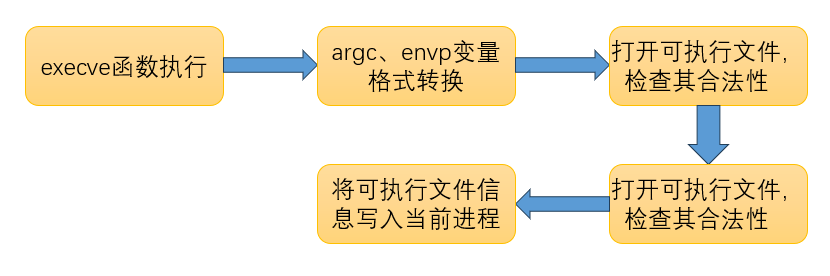
\includegraphics{figures/09-04-execve-流程图.png}}
    \caption{execve流程图}
\end{figure}

\subsubsection{代码详析}
下面将以NPUcore为例,讲述execve的实现。

1、函数的输入参数与返回值情况,已经在前面讲过,在此不过多赘述。
\begin{lstlisting}[language={Rust}, 
    caption={execve输入参数与返回值}]
pub fn sys_execve(
    pathname: *const u8,
    mut argv: *const *const u8,
    mut envp: *const *const u8,
) -> isize {
    //load_elf 成功
    SUCCESS
    //失败
    Err
}
\end{lstlisting}
2、将argv和envp变量字符串向量,通过循环,将*const *const u8转为Vec<String>数据类型。为后面的执行做准备。
\begin{lstlisting}[language={Rust}, 
    caption={execve参数转换}]
let mut argv_vec: Vec<String> = Vec::with_capacity(16);
    let mut envp_vec: Vec<String> = Vec::with_capacity(16);
    if !argv.is_null() {
        loop {
            let arg_ptr = match translated_ref(token, argv) {
                Ok(argv) => *argv,
                Err(errno) => return errno,
            };
            if arg_ptr.is_null() {
                break;
            }
            argv_vec.push(match translated_str(token, arg_ptr) {
                Ok(arg) => arg,
                Err(errno) => return errno,
            });
            unsafe {
                argv = argv.add(1);
            }
        }
    }
    if !envp.is_null() {
        loop {
            let env_ptr = match translated_ref(token, envp) {
                Ok(envp) => *envp,
                Err(errno) => return errno,
            };
            if env_ptr.is_null() {
                break;
            }
            envp_vec.push(match translated_str(token, env_ptr) {
                Ok(env) => env,
                Err(errno) => return errno,
            });
            unsafe {
                envp = envp.add(1);
            }
        }
    }
\end{lstlisting}
3、debug 层信息输出
\begin{lstlisting}[language={Rust}, 
    caption={execve的debug信息}]
debug!(
    "[exec] argv: {:?} /* {} vars */, envp: {:?} /* {} vars */",
    argv_vec,
    argv_vec.len(),
    envp_vec,
    envp_vec.len()
);
\end{lstlisting}
4、准备将 ELF 文件的内容载入当前进程,要对读取的文件做以下检查:
\begin{itemize}
    \item 文件大小大于等于 4
    \item 同时,ELF文件以 4 位魔数"7fELF"开头,因此应检查文件首是否有此魔数。 
\end{itemize}

\begin{lstlisting}[language={Rust}, 
    caption={对elf文件检查}]
match working_inode.open(&path, OpenFlags::O_RDONLY, false) {
    Ok(file) => {
        if file.get_size() < 4 {
            return ENOEXEC;
        }
        let mut magic_number = Box::<[u8; 4]>::new([0; 4]);
        // this operation may be expensive... I'm not sure
        file.read(Some(&mut 0usize), magic_number.as_mut_slice());
        let elf = match magic_number.as_slice() {
            b"\x7fELF" => file,
            b"#!" => {
                let shell_file = working_inode
                    .open(DEFAULT_SHELL, OpenFlags::O_RDONLY, false)
                    .unwrap();
                argv_vec.insert(0, DEFAULT_SHELL.to_string());
                shell_file
            }
            _ => return ENOEXEC,
        };

\end{lstlisting}
5、真正的载入过程。 loaf_elf 将当前的elf文件内容覆盖当前的进程。show_frame_consumption! 宏输出对应的信息。
\begin{lstlisting}[language={Rust}, 
    caption={execve载入可执行文件}]
let task = current_task().unwrap();
        show_frame_consumption! {
            "load_elf";
            if let Err(errno) = task.load_elf(elf, &argv_vec, &envp_vec) {
                return errno;
            };
        }
        // should return 0 in success
        SUCCESS
    }
    Err(errno) => errno,
}

\end{lstlisting}
6、深入load_elf()函数,了解execve的核心实现

可以很直观的发现,execve调用的elf载入函数load_elf()与
os::task::task::TaskControlBlock pub fn new(elf: FileDescriptor) -> Self 
第一个进程初始化函数的整体内容是比较相似的,都包括
\begin{itemize}
    \item 将elf文件映射到内存地址空间中
    \item 分配用户态资源
    \item 设置tcb信息
\end{itemize}
这些核心步骤。读者学习的时候不妨比照来阅读学习。

与new函数不同的是,load_elf会在原有的函数基础之上,进行部分信息的覆写。
首先,load_elf会覆写新进程的trap_cx对应的内容,并将其地址写入新进程的trap_cx_ppn中。

\begin{lstlisting}[language={Rust}, 
    caption={load_elf信息覆写-1}]
 // initialize trap_cx
    let trap_cx = TrapContext::app_init_context(
        if let Some(interp_entry) = elf_info.interp_entry {
            interp_entry
        } else {
            elf_info.entry
        },
        user_sp,
        KERNEL_SPACE.lock().token(),
        self.kstack.get_top(),
        trap_handler as usize,
    );
    // **** hold current PCB lock
    let mut inner = self.acquire_inner_lock();
    // update trap_cx ppn
    inner.trap_cx_ppn = (&memory_set)
        .translate(VirtAddr::from(self.trap_cx_user_va()).into())
        .unwrap()
        .ppn();
    *inner.get_trap_cx() = trap_cx;
\end{lstlisting}

第二,刷新子进程tid,堆指针等信息

\begin{lstlisting}[language={Rust}, 
    caption={load_elf信息覆写-2}]
// clear clear_child_tid
inner.clear_child_tid = 0;
// clear robust_list
inner.robust_list = RobustList::default();
// update heap pointers
inner.heap_bottom = program_break;
inner.heap_pt = program_break;
\end{lstlisting}

最后,刷新tcb的elf、fd表、memory_set、futex等信息,并返回载入成功的标识。

\begin{lstlisting}[language={Rust}, 
    caption={load_elf信息覆写-3}]
// track the change of ELF file
    *self.exe.lock() = elf;
    // flush cloexec fd
    self.files.lock().iter_mut().for_each(|fd| match fd {
        Some(file) => {
            if file.get_cloexec() {
                *fd = None;
            }
        }
        None => (),
    });
    // substitute memory_set
    *self.vm.lock() = memory_set;
    // flush signal handler
    for sigact in self.sighand.lock().iter_mut() {
        *sigact = None;
    }
    // flush futex
    self.futex.lock().clear();
    if self.tid_allocator.lock().get_allocated() > 1 {
        let mut manager = TASK_MANAGER.lock();
        // destory all other threads
        manager
            .ready_queue
            .retain(|task| (*task).tgid != (*self).tgid);
        manager
            .interruptible_queue
            .retain(|task| (*task).tgid != (*self).tgid);
    };
    Ok(())
\end{lstlisting}